\documentclass[10pt,a4paper,twocolumn]{article}
\usepackage{bachelorproject}
\usepackage{pgfplots}
\pgfplotsset{compat=1.12}
\usepackage{lmodern}
\usepackage{footmisc}
\usepackage{amsmath}
\usepackage{amssymb}
\usepackage{mathabx}
\usepackage{amsthm}
\usepackage{mathtools}


\usetikzlibrary{shapes,snakes}

\newcommand{\KP}[1]{%
	\begin{tikzpicture}[baseline=-\dimexpr\fontdimen22\textfont2\relax]
		#1
	\end{tikzpicture}%
}
\newcommand{\KPA}{%
	\KP{\filldraw[color=gray, fill=none, thick] circle (0.3);}%
}
\newcommand{\KPB}{%
	\KP{
		\draw[color=gray,thick] (-0.3,-0.3) -- (0.3,0.3);
		\draw[color=gray,thick] (-0.3,0.3) -- (-0.05,0.05);
		\draw[color=gray,thick] (0.05,-0.05) -- (0.3,-0.3);
	}%
}
\newcommand{\KPC}{%
	\KP{%
		\draw[color=gray,thick] (-0.3,-0.3) .. controls (0.05,0) .. (-0.3,0.3);
		\draw[color=gray,thick] (0.3,-0.3) .. controls (-0.05,0) .. (0.3,0.3);
	}%
}
\newcommand{\KPD}{%
	\KP{%
		\draw[color=gray,thick] (-0.3,0.3) .. controls (0,-0.05) .. (0.3,0.3);
		\draw[color=gray,thick] (-0.3,-0.3) .. controls (0,0.05) .. (0.3,-0.3);
	}%
}
\newcommand{\KPI}{%
	\KP{
		\draw[color=gray,thick] (-0.3,0.3) -- (0.3,-0.3);
		\draw[color=gray,thick] (-0.3,-0.3) -- (-0.05,-0.05);
		\draw[color=gray,thick] (0.05,0.05) -- (0.3,0.3);
	}%
}


\title{Nusos i el polinomi de Jones}
\author{Guillem Tutusaus Alcaraz, 1533701, 1533701@uab.cat}
%\text{Universitat Autònoma de Barcelona, Cerdanyola del Vallès}
\supervisors{Joan Porti Piqué}
\begin{document}
	\twocolumn[
	\maketitle
	\begin{@twocolumnfalse}
		\begin{abstract}
	Aquest és un document que tracta de donar una primera introducció a la teoria de nusos, estudiar alguns dels seus invariants algebràics més coneguts posant una ènfasis especial en el polinomi de Jones i classificar d'aquesta manera els nusos d'ordre més baix. Finalment, esmentarem algunes aplicacions.
	\vspace{6ex}
\end{abstract}

		%\tableofcontents
	\end{@twocolumnfalse}
	]
	
	\thispagestyle{firststyle}
	
	% !TEX root = thesis.tex
\renewcommand{\figurename}{Figura}
\renewcommand{\proofname}{Demostració}
\newtheorem{definition}{Definició}
\newtheorem{theorem}{Teorema}
\newtheorem{proposition}{Proposició}
\newtheorem{corolary}{Corol·lari}
\newtheorem{lemma}{Lema}

\section{Introducció}\label{sec:Introducció}
L'espècie humana té coneixement dels nusos desde temps prehistòrics. Començant per l'enregistrament d'informació, les xarxes de pesca i fins i tot per motius religiosos, els nusos han estat de gran importància per la seva utilitat i simbologia espiritual. Moltes obres d'art de cultures d'arreu del món presenten aquestes figures en les seves obres. Alguns exemples son la cultura Xinesa, Tibetana o Celta.\\

Els nusos comencen a tenir la seva presència dins el món de les matemàtiques a partir de l'any 1771 degut als treballs realitzats per Alexandre-Théophile Vandermonde el qual es dedicà a estudiar les propietats topològiques dels nusos en relació a la seva posició en l'espai. Treballs posteriors de Carl Friedrich Gau\ss$ $ qui va definir diverses propietats d'aquests objectes [\cite{knottheory}] van projectar aquesta teoria a la fama. L'any 1860 la teoria sobre l'atom en l'aether formulada per William Thomson va dur a Peter Guthrie Tait a la creació de les primeres taules de nusos. L'any 1885, aquest va publicar la primera taula amb tots els nusos de fins a deu creuaments, també va formular les conjectures que duen el seu nom.\\

A principis del segle XX, Max Dehn i J. W. Alexander van estudiar els nusos des del punt de vista de la teoria de grups i el seus invariants utilitzant grups d'homologia, cosa que va dur a la creació d'un dels primers invariants algebràics de la teoria, el polinomi d'Alexander.\\

A finals de l'any 1970, la incorporació de la geometria hiperbòlica en l'estudi dels nusos utilitzant el teorema de Geometrització de Thurston va permetre classificar aquests en funció de la seva mètrica, permetent l'ús de la geometria en la creació de nous invariants. El descobriment del polinomi de Jones per part de Vaughan Jones l'any 1984 [\cite{mathwithatwist}] juntament amb contribucions de Edward Witten i Maxim Kontsevich van revelar fortes relacions entre la teoria de nusos i mètodes matemàtics en mecànica estadística i teoria quàntica de camps. Una gran quantitat de invariant han estat inventats desde llavors utilitzant eines com els grups quàntics o la homologia de Floer.\\

En les darreres dècades, els científics han estat interessats en l'estudi dels nusos físics per tal de comprendre el nuament de l'ADN i de diferents polímers. Aquesta teoria s'utilitza també per determinar si una molècula és o no quiral. Finalment, la teoria de nusos pot ser crucial en la construcció dels primers ordinadors quàntics a través del model proposat per Alexei Kitaev [\cite{computingwithquantumknots}].\\

\subsection{Sobre els nusos}\label{subsec:sobreelsnusos}
Els nusos, son estructures presents en el nostre dia a dia. Podriem considerar un nus, en el sentit habitual, qualsevol de les figures següents.

\begin{figure}[h]
  \centering
  \includegraphics[width=0.401\linewidth]{img/nus simple.jpg}
  \includegraphics[width=0.535\linewidth]{img/Nus de Dara.jpg}
  \caption{D'esquerra a dreta: Nus simple (Overhand Knot en anglès) i Nus de Dara, nus celta símbol de la força.
  }\label{fig:exemples de nusos}
\end{figure}

El problema que tenen aquests nusos és que, aquests mantenen la seva forma a partir de la tensió i fricció que existeix entre les cordes que formen el nus. No és gaire difícil veure que un podria desfer aquests nusos de manera que acabariem obtenint una simple corda sense cap nus. És per això, que en matemàtiques és necessari considerar una definició més restrictiva d'aquest concepte per tal de preservar-ne l'estructura interna. Podriem pensar, que si uníssim els caps de les cordes de la Figura \ref{fig:exemples de nusos}, aleshores només tallant la corda seriem capaços de desfer el nus (això precisa de demostració!).
	% !TEX root = thesis.tex

\section{Algunes definicions i els objectius de la teoria de nusos}\label{sec:Algunes definicions i els objectius de la teoria de nusos}

De definicions de nus, parlant en termes matemàtics, n'hi ha diverses. Nosaltres considerarem la definició dins el camp de la topologia, d'on en reutilitzarem molta notació. A més, la teoria de nusos s'emmarca dins una teoria més general; la de links. Per tant, moltes vegades anirem mencionant resultats que també son vàlids per aquests objectes. La següent secció pretén donar unes primeres definicions pel que fa als nostres objectes d'estudi.

\begin{definition}\label{def: Definició de nus}
	Diem que $L$ és un \underline{link} de m components, o un m-link si és un subconjunt de $S^3$, o de $\mathbb{R}^3$, que consisteix en m corbes disjuntes, simples, tancades i lineals a trossos. Un 1-link és un \underline{nus}.
\end{definition}

La condició de lineal a trossos significa que les components de $L$ estan cadascuna d'elles feta d'un nombre finit de rectes col·locades una al costat de l'altra amb el principi d'una coincidint amb el final de l'altra. Aquesta condició evita la creació de nusos patològics que no presenten un comportament esperat. A aquests últims nusos se'ls anomena \textit{salvatges} i no seran estudiats en aquest treball. A la pràctica, quan representem nusos o links assumirem que hi ha tants segments rectes que cada component semblarà corba.\\

\begin{figure}
	\centering
	\includegraphics[width=0.9\linewidth]{img/wildknot.png}
	\caption{Exemple d'un nus salvatge.}\label{fig:nussalvatge}
\end{figure}

\textit{De què tracta la teoria de nusos?}
Una possible resposta és que la teoria de nusos pretén classificar el conjunt de possibles nusos. Donat un nus $K$, hom considera que aquest està inclòs, mitjançant una aplicació contínua, dins l'espai ambient tres dimensional $\mathbb{R}^3$ o equivalentment dins $S^3$, obtenim aleshores la teoria clàssica de nusos. Aquesta teoria pretén estudiar la col·locació de $K$ dins aquest espai. Classificar, en aquest cas vol dir considerar iguals sota certes condicions, que definirem més endavant.

\begin{figure}
	\centering
	\includegraphics[width=0.45\linewidth]{img/7_1.jpg}
	\includegraphics[width=0.45\linewidth]{img/anell borromeu.jpg}
	\caption{A l'esquerra el nus $7_1$ (més endavant explicarem el perquè del nom). A la dreta un 3-link conegut amb el nom d'anell Borromeu. 
	}\label{fig:exemplesdenusosenmatematiques}
\end{figure}

\begin{definition}
	Diem que un nus està \underline{desnuat} o que és el nus trivial, notacionalment $\ovoid$ si no presenta cap creuament en els segments de corda que el formen.
\end{definition}

\subsection{Equivalència entre nusos}\label{Equivalència entre nusos}

Expliquem ara què entem quan diem que dos nusos son el mateix.

\begin{definition}\label{def: Definició d'isotopia ambient}
	Diem que dos links $L$ i $L'$ a $S^3$ son equivalents si existeix una isotopia ambient entre ells.
\end{definition}
És a dir, si existeix una família d'homeomorfismes $h_t:S^3\rightarrow S^3$ per $t\in[0, 1]$ tal que $h_0=1$, $h_1=h$ i $(x, t)\mapsto(h_{t}x, t)$ és un homeomorfisme lineal a trossos de $S^3\times[0, 1]$ a $S^3$, llavors direm que $L$ i $L'$ son links equivalents. L'equivalència entre nusos és la mateixa que en la Definició \ref{def: Definició d'isotopia ambient} tenint present que en aquest cas només tenim una component. Observem que la distorsió no és del mateix link sinó de l'espai "ambient" $S^3$ en sí mateix. Definir nus equivalent d'aquesta manera evita que els creuaments que formen el nus o link puguin fer-se cada vegada més petits fins a desapareixer. D'aquesta manera, és possible moure tot $S^3$ de forma contïnua utilitzant $h_t$ per passar de $L$ a $L'$.

\subsection{Representació d'un nus en matemàtiques}\label{sec:Representació de nus}
Tenint present la definició de nus a partir d'ara en sentit matemàtic donada a la Definició \ref{def: Definició de nus}, un pot veure la dificultat d'estudiar aquest tipus d'objectes tres dimensionals en un llibre de text o bé en una pissarra. És per això, que per tal d'estudiar-los sovint es representen els nusos mitjançant el seu \textit{diagrama de nus}.\\

Considerant la projecció paral·lela (o axonomètrica) sobre l'eix $z$ en el pla $\mathbb{R}^2$ d'un nus qualsevol $K$, obtindrem una figura com en l'exemple \ref{fig:projecció d'un nus sobre R2}.\\

\begin{figure}
	\centering
		\resizebox{7.5cm}{!}{
			
			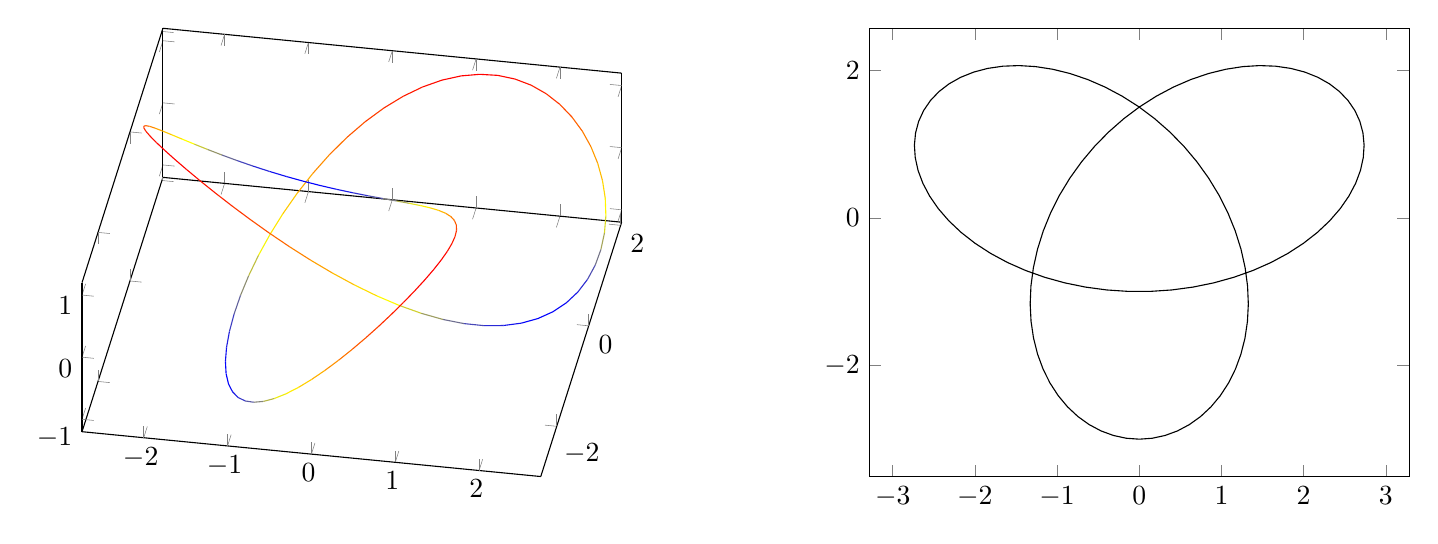
\begin{tikzpicture}
				
				\begin{scope}
					\begin{axis}
						\addplot [domain=-pi:pi,samples=120]({sin(deg(x))+2*sin(2*deg(x))},{cos(deg(x))-2*cos(2*deg(x))}); 
					\end{axis}
				\end{scope}
				
				\begin{scope}[xshift=-10cm]
					\begin{axis}
						[
						view={10}{60},
						]
						\addplot3[
						domain=-pi:pi,
						samples = 120,
						samples y=0,
						mesh
						]
						({sin(deg(x))+2*sin(2*deg(x))},
						{cos(deg(x))-2*cos(2*deg(x))},
						{-1*sin(3*deg(x))});
					\end{axis}
				\end{scope}
				
			\end{tikzpicture}
			
		}
	\caption{A l'esquerra el nus $3_1$ també conegut com Trefoil amb parametrització $(\sin t+2\sin 2t, \cos t-2\cos 2t,-\sin 3t)$. A la dreta, la seva projecció paral·lela sobre l'eix $z$.}\label{fig:projecció d'un nus sobre R2}
\end{figure}

Considerant aquesta projecció però, un perd informació sobre el propi nus, ja que cal saber quin segment de corda va per sobre i quin per sota alhora de creuar-se. Per tal de no perdre aquesta informació, el segment que passa per sota se'l dibuixa de forma discontínua mentre aquest passa sota el segment de corda que el creua.\\

\noindent
D'aquesta manera, la projecció del nus $3_1$ de la Figura \ref{fig:projecció d'un nus sobre R2} quedaria de la següent manera:

\begin{figure}[H]
	\resizebox{6.5cm}{!}{
		\begin{tikzpicture}[line width=0.5mm]
			\begin{scope}[rotate=270]
				\begin{knot}[
					consider self intersections=true,
					%  draft mode=crossings,
					flip crossing=2,
					only when rendering/.style={
						%    show curve controls
					}
					]
					\strand (0,2) .. controls +(2.2,0) and +(120:-2.2) .. (210:2) .. controls +(120:2.2) and +(60:2.2) .. (-30:2) .. controls +(60:-2.2) and +(-2.2,0) .. (0,2);
				\end{knot}
			\end{scope}
			
			\begin{scope}[xshift=-5cm, rotate=270]
				\begin{knot}[
					consider self intersections=false,
					%  draft mode=crossings,
					flip crossing=2,
					only when rendering/.style={
						%    show curve controls
					}
					]
					\strand (0,2) .. controls +(2.2,0) and +(120:-2.2) .. (210:2) .. controls +(120:2.2) and +(60:2.2) .. (-30:2) .. controls +(60:-2.2) and +(-2.2,0) .. (0,2);
				\end{knot}
			\end{scope}
		\end{tikzpicture}
	}
\end{figure}

Així doncs, considerant la projecció paral·lela sobre l'eix $z$ d'un nus $K$ qualsevol i disposant de la informació sobre els creuaments obtenim el que anomenarem \textit{diagrama de nus}, notacionalment $diag(K)$. Moltes vegades, en la literatura es fa un abús de llenguatge i notació, anomenant nus al que nosaltres anomenem diagrama de nus i fent servir $K$ i $diag(K)$ indistintament. D'aquí a no massa veurem que de fet, estudiar-ne les propietats d'un és equivalent a estudiar les de l'altre.\\
	% !TEX root = thesis.tex

\section{Els moviments de Reidemeister}\label{sec:Reidermeister}
Una primera aproximació per tal de distingir si dos nusos son diferent és veure quan son iguals. Aquesta és la inspiració darrera de la següent secció que tractarà sobre els moviments de Reidemeister i el Teorema central de la Teoria de Nusos.

\subsection{Moviments de Reidemeister}\label{subsec:Moviments de Reidemeister}
Motivats per la Secció \ref{Equivalència entre nusos}, un podria veure sense massa dificultat que cadascun dels moviments de la Figura \ref{fig:Moviments de Reidemeister} resulta en un diagrama de nus equivalent a l'original.\\

\begin{figure}[h]
	\centering
	\includegraphics[width=0.9\linewidth]{img/movimentsdereidemeister.png}
	\caption{De dalt a baix: Moviment de Tipus I, Tipus II i Tipus III  [\cite{SobreelsmovdeReide}]. Cal pensar que els segments lliures de corda s'uneixen a través d'un nus $K$.}\label{fig:Moviments de Reidemeister}
\end{figure}

A aquests tres tipus de moviments se'ls anomena moviments de Reidemeister. Al primer de tots se'l diu de Tipus I o \textit{twist} en anglès, al segon de Tipus II o \textit{poke} i al tercer de Tipus III o \textit{slide}.\\

\noindent
\textbf{Moviment de Tipus I o \textit{twist}:} També anomenat \textbf{RI} per abreujar notació, aquest tipus de moviment consisteix en "pessigar" la corda i amb el tros obtingut donar-li la volta (d'aquí el nom en anglès) fent un bucle com en el de la Figura \ref{fig:Moviments de Reidemeister}.\\

\noindent
\textbf{Moviment de Tipus II o \textit{poke}:} També anomenat \textbf{RII}. Aquest tipus de moviment consisteix en fer passar una de les dues cordes per sobre de l'altra. En anglès, la paraula \textit{poke} significa fer passar forçosament alguna cosa en una certa direcció i doncs en aquest cas es podria pensar que una de les dues cordes s'ha fet passar per sobre de l'altra.\\

\noindent
\textbf{Moviment de Tipus III o \textit{slide}:} També anomenat \textbf{RIII}. Aquest tipus de moviment consisteix en, com el nom en anglès indica, fer lliscar una de les tres cordes d'una banda a l'altra de la intersecció entre les dues cordes restants. En la Figura \ref{fig:Moviments de Reidemeister} podem veure com el segment de corda horitzontal llisca de dalt a baix del creuament entre les altres dues cordes.\\

La Figura \ref{fig:movimentsdereidemeisteraltrefoil} mostra el nus $3_1$ juntament amb aquest mateix havent aplicat cadascun dels moviments anteriors.\\

\begin{figure}
	\centering
	\includegraphics[width=\linewidth]{img/moviments de reidemeister (2).jpg}
	\caption{Moviments de Reidemeister aplicats al nus $3_1$. D'esquerra a dreta i de dalt a baix: Nus $3_1$, nus $3_1$ havent aplicat un moviment RI, RII i RIII respectivament. Per aplicar RIII hem hagut d'aplicar RI abans ja que no es possible aplicar directament RIII en aquest cas.}\label{fig:movimentsdereidemeisteraltrefoil}
\end{figure}

Continuant amb el que hem vist, no és massa difícil veure que aplicant una seqüència finita de moviments RI, RII o RIII a un diagrama de nus qualsevol, el nus obtingut és equivalent a l'original.

\subsection{El Teorema central de la Teoria de Nusos}\label{sec:teoremacentraldelateoria}

L'any 1930, Kurt Reidemeister demostrà que l'implicació contrària també és certa, és a dir que si dos diagrames de nusos qualssevol son equivalents, aleshores sempre podem trobar una seqüència finita de moviments de Reidemeister de manera que podem transformar un diagrama de nus en l'altre. Aquest resultat va donar lloc al teorema central de la teoria.

\begin{theorem}\label{teo:teoremadeReidemeister}
   $diag(K)$ i $diag(K')$ son equivalents si i només si, existeix una seqüència finita de moviments RI, RII o RIII que passa d'un a l'altre.
\end{theorem}

Una demostració del teorema original es pot trobar a [\cite{knotknotes}]. Aquesta demostració es troba fora de l'objectiu del treball --- i per això s'ha optat a no reproduïr-la --- però en essència aquesta demostració fa ús del fet que un pot generar nusos equivalents a l'original afegint triangles als costats d'un nus poligonal.\\

\begin{figure}
	\centering
	\includegraphics[width=0.9\linewidth]{img/culprit-knot.png}
	\caption{Com es pot observar en l'exemple, el nus de Culprit és equivalent al nus trivial. Mitjançant la seqüència de moviments següent podem passar de l'un a l'altra. D'esquerra a dreta i de dalt a baix: RII, RIII+RIII, RII, RIII, RI+RII, RII, RII, RII, RI, [\cite{culpritknot}].}\label{fig:culpritknot}
\end{figure}

El Teorema \ref{teo:teoremadeReidemeister} doncs, posa en evidència el fet que parlar d'equivalència entre nusos o d'equivalència entre diagrames de nusos és el mateix, doncs aquests estan en correspondència a través de la Secció \ref{sec:Representació de nus}.\\

D'aquesta manera i fent referència al mencionat anteriorment, a partir d'ara farem un abús de llenguatge i notació dient nus $K$ indistintament sense donar importància al fet de si ens referim al nus o al seu diagrama.
	% !TEX root = thesis.tex

\section{Propietats sobre nusos}\label{sec:Propietats_sobre_nusos}

En aquesta secció posarem de manifest diferents propietats d'un nus que més endavant tindran importància en la seva classificació.

\begin{definition}\label{def:ordre}
	Anomenem \underline{ordre} de $K$, $O(K)$ al mínim nombre de creuament que $K$ pot arribar a presentar donat un diagrama qualsevol.
\end{definition}

La Figura \ref{fig:culpritknot} demostra que l'ordre del nus Culprit és zero ja que aquest sempre és un nombre positiu. Tampoc és molt difícil veure que donat un nus $K$ qualsevol a aquest se li pot afegir creuaments mitjançant moviments RI, no obstant $O(K)$ es manté contant.

\begin{definition}\label{def:nusemmirallat}
	Diem que un nus és l'\underline{emmirallat} $\overline{K}$ d'un altre nus $K$ si aquest primer s'obté a partir de l'original canviant tots els creuaments de sobrepassos a sotapassos i a la inversa.
\end{definition}

La Figura \ref{fig:nus emmirallat} mostra un exemple d'un nus emmirallat.\\

\begin{figure}
	\resizebox{6.5cm}{!}{
		\begin{tikzpicture}[line width=0.5mm, use Hobby shortcut]
			\begin{scope}
				\begin{knot}[
					consider self intersections=true,
					%  draft mode=crossings,
					ignore endpoint intersections=false,
					flip crossing/.list={1,5,6},
					only when rendering/.style={
						%    show curve endpoints
					}
					]
					\strand ([closed]0,0) .. (1.5,1) .. (.5,2) .. (-.5,1) .. (.5,0) .. (0,-.5) .. (-.5,0) .. (.5,1) .. (-.5,2) .. (-1.5,1) .. (0,0);
				\end{knot}
				\path (0,-.7);
			\end{scope}
			
			\begin{scope}[xshift=-5cm]
				\begin{knot}[
					consider self intersections=true,
					%  draft mode=crossings,
					ignore endpoint intersections=false,
					flip crossing/.list={3,4},
					only when rendering/.style={
						%    show curve endpoints
					}
					]
					\strand ([closed]0,0) .. (1.5,1) .. (.5,2) .. (-.5,1) .. (.5,0) .. (0,-.5) .. (-.5,0) .. (.5,1) .. (-.5,2) .. (-1.5,1) .. (0,0);
				\end{knot}
				\path (0,-.7);
			\end{scope}
		\end{tikzpicture}
	}
	\caption{A l'esquerra el nus $4_1$ o Figure Eight en Anglès. A la dreta, el seu nus emmirallat.}\label{fig:nus emmirallat}
\end{figure}

D'aquesta manera, si un nus $K$ és equivalent a $\overline{K}$, llavors diem que és \textit{amfiquiral}, sinó diem que és \textit{quiral}. El nus $4_1$ de la Figura \ref{fig:nus emmirallat} és un exemple de nus amfiquiral, però no sempre és veritat que un nus $K$ sigui equivalent a $\overline{K}$ com veurem més endavant.

\begin{definition}\label{def:nusinvers}
	Diem que un nus és l'\underline{invers} $rK$ d'un altre nus $K$ si aquest primer s'obté a partir de l'original canviant-ne l'orientació.
\end{definition}

És clar que un nus pot ser orientat de dues maneres diferents, escollir una d'aquestes orientacions és informació extra sobre el nus que pot o no ser donada. De manera similar a la Definició \ref{def:nusemmirallat}, no sempre un nus és equivalent al  seu invers.

\begin{figure}
	\centering
	\includegraphics[width=0.6\linewidth]{img/orientació.png}
	\caption{Les dues úniques orientacions del nus trivial. És evident que aquests dos diagrames son equivalents.}\label{fig:nusorientat}
\end{figure}

\begin{definition}
	Diem que un nus $K$ és \underline{primer} si no és el nus trivial i si $K=K_1+K_2$ implica que $K_1$ o $K_2$ és el nus trivial.
\end{definition}

En aquest cas, el símbol $+$ fa referència a l'operació suma. Donats dos nusos orientats $K$ i $K'$, aquests poden ser sumats posant-los un al costat de l'altre i unint-los de manera que es preservi l'orientació. Aquesta operació està ben definida sota equivalència. A més, és commutativa, associativa, té element neutre i es comporta de forma similar al producte de nombres enters. De fet, caldria pensar en la suma de nusos com la suma conexa de varietats desenvolupada en un curs fonamental de topologia.\\

\begin{figure}
	\centering
	\includegraphics[width=0.9\linewidth]{img/nussuma.png}
	\caption{Suma de dos nusos qualssevol.}\label{fig:nussuma}
\end{figure}

La Figura \ref{fig:knotable} és una taula que conté tots els nusos primers de fins a 9 creuaments. Cadascun rep un nom conformat per un parell de nombres; el primer de tots correspon al seu ordre i el segon és un subíndex històricament assignat a aquell nus en concret. Les primeres tabulacions que es coneixen van fer-se per Tait l'any 1860 mentre aquest estudiava l'àtom. Aquesta taula negligeix el fet que possiblement un mateix nus $K$ sigui diferent a $\overline{K}$, $rK$ o $\overline{rK}$. D'aquesta manera, cada nus de la taula correspon a un, dos o quatre nusos de $S^3$ mitjançant les operacions definides a \ref{def:nusemmirallat} i \ref{def:nusinvers}.

\begin{figure}
	\centering
	\includegraphics[width=0.9\linewidth]{img/knottable.png}
	\caption{Taula de nusos fins a ordre 9.}\label{fig:knotable}
\end{figure}

\begin{definition}\label{def:nusalternat}
	Diem que $K$ és un nus \underline{alternat} si a mesura que anem recorrent el nus, els creuaments alternen de sobrepassos a sotapassos.
\end{definition}

El nus $4_1$ n'és un exemple. De fet, cal anar fins a $8_{19}$ per trobar el primer nus no alternat i doncs això és una conseqüència del baix ordre dels nusos. Es pot veure que donat un ordre qualsevol, sempre existeix com a mínim un nus alternat. Ara bé, aquests disminueixen exponencialment a mesura que incrementem l'ordre del nus. Aquesta classe de nusos tenen bones propietats.
	% !TEX root = thesis.tex

\section{Alguns invariants algebràics}\label{sec:Invariantsalgebraics}

El Teorema \ref{teo:teoremadeReidemeister} dona un mètode per saber quan dos nusos son equivalents, aquest resultat però no permet distingir quan dos nusos son diferents. D'aquesta manera per exemple, encara no sabem que $\ovoid\neq 3_1$. Per això que és necessari la creació d'invariants que ens permetin realitzar aquesta tasca.\\

Recordem que un invariant és un objecte ben definit, ja sigui un número, polinomi, grup, etcètera; que podem associar a un nus qualsevol, de manera que si tenim dos nusos amb diferent valor per aquest invariant, llavors segur que els dos nusos son diferents.

\subsection{L'Ordre}\label{sec:ordrecomainvariant}

Com ja podriem haver esperat, l'ordre d'un nus és un exemple d'invariant. Nusos amb diferent ordre no poden ser equivalents. Aquest invariant però és intractable a nivell pràctic pel fet d'haver de considerar el mínim nombre de creuaments donats tots els diagrames d'aquest.\\

\begin{proposition}
	L'ordre d'un nus és un invariant.
\end{proposition}

\begin{proof}
	Sigui $K$ un nus qualsevol amb diagrama $diag(K)$. Siguin $K_1, K_2, K_3, \dots$ nusos equivalents a $K$ amb els seus respectius diagrames formats a partir de diferents transformacions de $K$. D'entre aquests nusos, tenim un nus $K_k$ que té el mínim nombre de creuaments $x$. Definim $O(K)=O(K_k)=x$. Evidentment, $x=O(K_1)=O(K_2)=O(K_3)=\dots$. Ara, quan transformem el nus $K$ en un nus equivalent, com aquest està a la llista de nusos, aquest també pot ser transformat en $K_k$ on $O(K_k)=x$.
\end{proof}

\subsection{El Nombre de Desnuament}\label{sec:desnuamentcomainvariant}

\begin{definition}\label{def:desnuament}
	Diem que $u(K)$ és el \underline{nombre de desnuament} del nus $K$ si aquest és el mínim nombre de canvis en els creuaments d'un diagrama de nus necessaris per tal d'aconseguir el nus trivial. $$u(K)=\min\{u(D)|\text{D diagrama de K}\}$$
\end{definition}

El nombre de desnuament és també un invariant. Aquest però, de la mateixa manera que passa amb l'ordre és intractable a nivell pràctic. Intuïtivament, si $K$ és una corba a $S^3$, llavors $u(K)$ és el mínim nombre de vegades que $K$ ha de passar per sí mateix per aconseguir el nus trivial.

\begin{proposition}\label{prop:nombrededesnuament}
	Donat un nus $K$ qualsevol, aquest sempre pot ser desnuat, i.e. $u(K)$ és finit.
\end{proposition}

\begin{proof}
	Entenem per \textit{moviment local} un canvi en els creuaments d'un nus com en el de la Figura \ref{fig:movimentlocal} passant de sobrepassos a sotapassos o a la inversa. D'aquesta manera, recorrent $K$ d'acord amb una orientació qualsevol i fent moviments locals canviant sotapassos a sobrepassos a mesura que aquests van apareixen sense modificar els creuaments que ja haguem visitat ja ho tindriem.
\end{proof}

\begin{figure}
	\centering
	\includegraphics[width=0.6\linewidth]{img/movimentlocal.png}
	\caption{Moviments locals que es poden realitzar en qualsevol creuament d'un nus. A la imatge de l'esquerra, el tros de corda que va de  Sud-Oest fins a Nord-Est passa per sobre de la corda que el creua i doncs en aquest sentit diem que la sobrepassa. A la dreta, aquesta mateixa corda creua per sota i doncs diem que la sotapassa.}\label{fig:movimentlocal}
\end{figure}

\begin{proposition}
	Sigui $K$, $K'$ dos nusos qualssevol, llavors $u(K+K')\leq u(K)+u(K')$
\end{proposition}

\begin{proof}
	És clar que per tal de desnuar $K+K'$ només fa falta desnuar $K$ i $K'$.
\end{proof}

L'altre desigualtat és de fet un problema obert.\\

De fet, coneixer el nombre de desnuament d'un nus pot pensar-se com l'objectiu d'aquesta teoria. Si veiem que un nus $K$ no és el nus trivial i que un moviment local en algun dels creuaments dona com a resultat el nus trivial, llavors segur que $u(K)=1$. Així doncs, d'aquí a no massa estarà clar que $u(3_1)=u(4_1)=1$. No obstant, actualment encara hi ha una gran quantitat de nusos com per exemple $10_{11}$ dels quals se'ls hi desconeix el nombre de desnuament. Per aquest últim es creu que es troba entre dos i tres.\\

Existeixen més resultats que poden ser útils alhora de diferenciar nusos, 

\subsection{El Gènere}\label{sec:generescomainvariant}

Veurem ara que tot link a $S^3$ es pot veure com la frontera d'una superfície immersa en $S^3$. Aquestes superfícies poden ser utilitzades per estudiar el link.

\begin{definition}\label{def:superficiedeseifert}
	Una \underline{superfície de Seifert} $S$ per un link $L$ orientat de $S^3$ és una superfície compacta, connexa i orientable, $S\subset S^3$ de manera que la seva frontera és $L$, i.e. $\partial S=L$.
\end{definition}

No es gens evident a partir de la Definició \ref{def:superficiedeseifert} que aquests objectes hagin d'existir i encara menys evident com es construeixen. A continuació veurem que de fet, existeix un algorisme per construir-los. Exemples d'aquestes superfícies son com les de la Figura \ref{fig:superficiedeseifert}. \\

És evident que tota superfície compacta connexa i orientada amb frontera dins $S^3$ és un exemple d'un link. Una superfície és no orientable si conté una banda de Möbius. Algunes superfícies poden ser construïdes amb un link qualsevol com a frontera de la següent manera: Pintant de color blanc i negre seguint un patró com el d'un taulell d'escacs les regions de $S^2$ que formen el complement del diagrama d'un link. Considerant totes les regions d'un mateix color i juntant-les per bandes amb una mitja volta arribem a obtenir un objecte com el de la Figura \ref{fig:trefoilseifert}.\\

\begin{figure}
	\centering
	\includegraphics[width=0.6\linewidth]{img/seifertsurface.png}
	\caption{Exemple d'una superfície de Seifert per $5_2$.}\label{fig:superficiedeseifert}
\end{figure}

\begin{figure}
	\centering
	\includegraphics[width=0.6\linewidth]{img/trefoilseifert.png}
	\caption{Dos diagrames del nus $3_1$ pintats com indiquen les instruccions. Com es pot observar, la superfície de l'esquerra és no orientable al ser una cinta de Möbius amb tres mitjes voltes, la de la dreta, en canvi, sí; i doncs és una superfície de Seifert com haviem vist a la Definició \ref{def:superficiedeseifert}. Notem doncs que diagrames diferents d'un mateix nus poden o no donar lloc a una superfície de Seifert.}\label{fig:trefoilseifert}
\end{figure}

Tot i que aquest mètode pot donar com a resultat una superfície de Seifert, en general aquest no té perquè ser el cas. Herbert Seifert demostrà l'existència d'aquests objectes i donà un algorisme --- que duu el seu mateix nom --- per trobar-les [\cite{seifert}].

\begin{theorem}\label{theo:existenciadesuperficiesdeseifert}
	Tot link orientat $L$ a $S^3$ té una superfície de Seifert.
\end{theorem}

\begin{proof}
	Sigui $diag(L)$ un diagrama orientat de $L$ qualsevol i sigui $\widehat{diag(L)}$ aquest darrer diagrama modificat segons indica la Figura \ref{fig:movimentsdeseifert}, llavors $\widehat{diag(L)}$ és el mateix que $diag(L)$ excepte en un entorn prou petit de cada creuament on aquest ha sigut eliminat de la única manera coherent amb l'orientació del nus. Aquest $\widehat{diag(L)}$ és doncs una unió disjunta de corbes orientades simples i tancades dins $S^2$. D'aquesta manera, $\widehat{diag(L)}$ és la frontera de la unió d'un nombre de discs disjunts. Considerant que aquests disc es troben al mateix nivell, excepte si aquests estan un contingut en l'altre --- en aquest cas el disc de dins es considerarà a sobre l'altre disc --- juntem els discs mitjançant bandes amb una mitja volta als mateixos llocs on hi havia els creuaments. Això forma una superfície orientada amb $L$ com a frontera. Cada disc rep la orientació induïda per $\widehat{diag(L)}$ i les bandes que uneixen els diferents discos van alternant aquesta orientació.
\end{proof}

\begin{figure}
	\centering
	\includegraphics[width=0.6\linewidth]{img/seifert.png}
	\caption{Moviments utilitzats en l'algorisme de Seifert. Quan ens trobem amb un creuament, resoldrem aquest com mostra la imatge central reseguint el nus o link com indica la seva orientació.}\label{fig:movimentsdeseifert}
\end{figure}

En la demostració del Teorema \ref{theo:existenciadesuperficiesdeseifert}, $\widehat{diag(L)}$ era una col·lecció disjunta de corbes simples i tancades construïdes a partir de $diag(L)$. Aquestes corbes s'anomemen \underline{cercles de Seifert} del $diag(L)$. La Figura \ref{fig:cerclesdeseifert} dona un exemple d'aquesta.\\

\begin{figure}
	\centering
	\includegraphics[width=\linewidth]{img/cerclesdeseifert.png}
	\caption{Exemple amb la construcció de $\widehat{diag(3_1)}$ a partir d'un diagrama de $3_1$ qualsevol.}\label{fig:cerclesdeseifert}
\end{figure}

Una superfície de Seifert per la Figura \ref{fig:cerclesdeseifert} s'aconsegueix superposant les dues corbes disjuntes una a sobre l'altra i unir-les mitjançant tres bandes amb una mitja volta cadascuna en els creuaments. Evidentment, aquest algorisme dona lloc a una superfície de Seifert. Donat un diagrama qualsevol de $L$ però, aquesta no té perquè ser única. Tampoc té perquè ser la més senzilla donat un diagrama qualsevol.

\begin{figure}
	\centering
	\includegraphics[width=0.6\linewidth]{img/superficiedeseifert.png}
	\caption{superfície de Seifert pel nus $3_1$ obtinguda unint els discos a través de bandes amb una mitja volta. Una senzilla comprovació demostra que la frontera de la superfície és el mateix nus.}\label{fig:superficiedeseifert2}
\end{figure}

\begin{definition}\label{def:genere}
	El \underline{gènere} $g(K)$ d'un nus $K$ es defineix com $$g(K)=\min\{g(S)| \text{S superfície de Seifert de K}\}$$ Direm que una superfície de Seifert $S$ amb $K$ com a frontera és \textit{minimal} si $g(S)=g(K)$.
\end{definition}

\begin{proposition}
	El gènere d'un nus és invariant.
\end{proposition}

\begin{proof}
	Considerem una superfície de Seifert minimal $S$ que té per frontera $K$. Com $K$ és equivalent a $K'$ llavors ha d'existir un homeomorfisme $h:S^3\rightarrow S^3$ de manera que $h(K)=K'$. Llavors, $h(S)$ és una superfície de Seifert que té per frontera $K'$ i $g(h(S))=g(S)=g(K)$. A més, $h(S)$ és una superfície de Seifert minimal que té $S'$ per frontera i per tant $g(K)=g(K')$. Si $h(S)$ no fos una superfície de Seifert minimal de $K'$, llavors existiria una superfície de Seifert minimal $S'$ que tindria $K'$ per frontera i tal que $g(S')<g(h(S))$ i per tant $h^{-1}(S')$ seria una superfície de Seifert amb $K$ per frontera amb gènere menor que $g(S)$, però això no pot ser ja que $S$ és minimal.
\end{proof}

Com en aquest cas $K$ és un nus, $S$ només té una component de frontera de manera que com a superfície abstracta és un disc amb un nombre concret de "mànecs". A aquest nombre se l'anomena gènere. Més precisament, el gènere de $S$ és

\begin{equation}\label{eq:generedunasuperficie}
	g(S)=\frac{1}{2}(1-\mathcal{\chi}(S))
\end{equation}

on $\mathcal{\chi}$ és la característica d'Euler de $S$. La característica d'Euler es pot definir paral·lelament com el nombre de vèrtex menys el nombre de costats més el nombre de triangles en qualsevol triangulació de $S$.\\

Si $diag(K)$ té $n$ creuament i $s$ cercles de Seifert, llavors $\mathcal{\chi}(S)=s-n$ de manera que

\begin{equation}\label{eq:cotasuperiorgenere}
	g(K)\leq \frac{1}{2}(n-s+1)
\end{equation}

Aquest invariant té un millor tractament que els vistos anteriorment. Donem ara una caracterització del nus trivial en termes del gènere.

\begin{proposition}
	$K$ és el nus trivial si i només si $g(K)=0$.
\end{proposition}

\begin{proof}
	Si $K$ és el nus trivial, llavors un disc amb frontera $K$ és clarament una superfície de Seifert minimal amb $K$ per frontera. I com que un disc és una esfera amb un component de frontera deduïm que $g(K)=g(S^2)=0$. Alternativament, si $K$ és tal que $g(K)=0$, llavors existeix una superfície de Seifert minimal $S$ amb $g(S)=0$, d'aquesta manera $S$ és una esfera amb una component per frontera, i.e. un disc.
\end{proof}

Seguint amb l'exemple del nus $3_1$, llavors es veu clarament que $g(3_1)=1$. Per tant, ja sabem que $3_1\neq\ovoid$. De manera similar un pot arribar a calcular els gèneres d'un gran nombre de nusos. El problema amb aquest mètode és que l'Equació \ref{eq:cotasuperiorgenere} dona una cota superior per aquest gènere i per tant, a mesura que incrementem el nombre de creuaments és possible que el gènere pugui prendre un nombre finit de valor diferents entre ells. Per exemple, un exercici senzill demostra que $g(8_{20})\leq2$ i doncs pot ser 1 o bé 2.

\subsubsection{Additivitat i aplicacions}

\begin{theorem}\label{teo:sumabilitatdelgenere}
	Donats dos nusos $K$ i $K'$, $$g(K+K')=g(K)+g(K')$$
\end{theorem}

\begin{proof}
	Comencem veient $g(K+K')\leq g(K)+g(K')$. Considerem que $K$ i $K'$ estan separats per un pla i considerem les superfícies de Seifert minimals de tots dos nusos $S$ i $S'$ ($S$ i $S'$ també estan separades pel pla). Donem una orientació a $K$ i $K'$ i considerem la seva suma assegurant-nos que $K+K'$ no intersecti $Int(S)$ ni $Int(S')$. Considerem ara una banda $B$ que conecta $K$ i $K'$ que té per frontera els dos segments de corda introduïts al considerar la suma $K+K'$ i de tal manera que $B$ no intersecta $Int(S)$ ni $Int(S')$. D'aquesta manera, $B$ conecta $S$ i $S'$ i doncs $C=S\cup S'\cup B$ és una superfície de Seifert per $K+K'$. Finalment com $g(C)=g(S)+g(S')=g(K)+g(K')$ tenim $g(K+K')\leq g(K)+g(K')$. L'altre desigualtat es pot trobar a AAAAAAAAAAAAAAAAAAAAAA
\end{proof}

A partir del Teorema \ref{teo:sumabilitatdelgenere} obtenim un seguit de resultats:

\begin{corolary}
	Cap nus tret del nus trivial té oposat respecte la suma. És a dir, que si $K+K'=\ovoid$, llavors $K=K'=\ovoid$.
\end{corolary}

\begin{proof}
	Suposem que existeix $K$ i $K'$ amb almenys un d'ells diferent del nus trivial de manera que $K+K'=\ovoid$, llavors en virtut del Teorema \ref{teo:sumabilitatdelgenere}
	\begin{align*}
		&g(K+K')=g(K)+g(K')\\
		&0=g(K)+g(K')
	\end{align*}
	Com que el gènere d'un nus és un nombre positiu, tenim que $g(K)=g(K')=0$.
\end{proof}

\begin{corolary}
	Hi ha un nombre infinit de nusos diferents.
\end{corolary}

\begin{proof}
	Sigui $K$ un nus no trivial qualsevol i $\sum^{n}K$ la suma de $n$ còpies d'aquest. Veiem que si $n\neq m$, llavors $\sum^{n}K\neq\sum^{m}K$. Suposem que $\sum^{n}K=\sum^{m}K$, aleshores $\sum^{n}g(K)=\sum^{m}g(K)$. Sense pèrdua de generalitat podem suposar que $m>n$, d'aquesta manera $\sum^{m-n}g(K)=0$ cosa que implica $K=\ovoid$. Contradicció amb el fet que $K$ no pot ser trivial.
\end{proof}

\begin{corolary}
	Un nus $K$ amb gènere $1$ és primer.
\end{corolary}

\begin{proof}
	Sigui $K$ un nus amb $g(K)=1$ i expressem aquest com a suma de nusos $K_1$ i $K_2$, llavors $1=g(K_1)+g(K_2)$ i per tant $g(K_1)=0$ o al revés.
\end{proof}

\begin{corolary}
	Tot nus $K$ pot ser expressat com a suma finita de nusos primers.
\end{corolary}

\begin{proof}
	Si $K$ és primer, llavors el resultat és obvi. Suposem ara que $K$ no sigui un nus primer. Per definició, existeixen $K_1$ i $K_2$ tots dos diferents del nus trivial de manera que $K=K_1+K_2$ i del Teorema \ref{teo:sumabilitatdelgenere} sabem que $g(K_1),g(K_2)<g(K)$. Ara, fent el mateix procés amb $K_1$ i $K_2$ podem concloure que $K$ és suma de nusos primers.
\end{proof}

\begin{corolary}
	Existeixen nusos amb un nombre de creuaments arbitràriament gran.
\end{corolary}

\begin{proof}
	Sigui $K$ un nus qualsevol, com que el nombre de cercles de Seifert sempre serà com a mínim $1$, utilitzant l'Equació \ref{eq:cotasuperiorgenere} tenim $$g(K)\leq \frac{n}{2}$$ on $n$ és el nombre de creuaments del diagrama de $K$. Considerem ara un nus no trivial i $K_m=\sum^{m}K$ la suma de $m$ còpies de $K$. Llavors, $$m\leq g(K_m)\leq \frac{c(K_m)}{2}$$ on $c(K_m)$ és el nombre de creuaments de la suprfície de Seifert de $K_m$. A mesura que $m$ s'acosta a infinit, també ho fa $c(K_m)$.
\end{proof}

Cal remarcar que existeixen cotes inferiors pel gènere d'un nus qualsevol [\cite{lowerbound}] i que hi ha classes de nusos amb molt bones propietats pel que fa el seu gènere. Nosaltres però al no fer-nos falta, ens limitarem a fer-ne menció i classificarem els nusos d'ordre més baix utilitzant només els resultats vistos.\\

La Figura \ref{fig:genus} mostra una taula per al gènere d'un nus primer de fins a $7$ creuaments.

\begin{figure}
	\centering
	\includegraphics[width=\linewidth]{img/genus.png}
	\caption{Gènere de tots dels nusos primers de fins a $7$ creuaments.}\label{fig:genus}
\end{figure}
	% !TEX root = thesis.tex

\section{El polinomi de Jones}\label{sec:El polinomi de Jones}

El descobriment del \textit{polinomi de Jones} per part de Vaughan Jones l'any 1984 [\cite{jonesoriginal}] dona una manera d'associar a cada nus o link un polinomi de Laurent amb coeficients enters. Aquesta correspondència es fa mitjançant un diagrama de link qualsevol. La teoria de Jones es fonamenta en el fet que si fem un moviment RI, RII o RIII al diagrama del link, aquest polinomi no canvia i doncs és un invariant sota moviments de Reidemeister. El polinomi per un link és doncs independentment del diagrama d'aquest. De manera que si podem veure que dos diagrames de links no tenen el mateix polinomi, llavors segur que aquests son diferents.\\

La manera més simple per definir-lo és mitjançant un altre tipus de polinomi; el \textit{polinomi de Kauffman} descobert per Louis Kauffman.\\

\begin{definition}
	El \underline{polinomi de Kauffman} de $L$, $\langle L\rangle$ és un polinomi de Laurent amb coeficients enters i indeterminada $A$ que podem associar a tot diagrama d'un link a $S^2$ de la següent manera:
	\begin{enumerate}
		\item\label{item:i} $\left\langle\KPA\right\rangle=1$
		\item\label{item:ii} $\left\langle L \cup \KPA\right\rangle=(-A^{-2}-A^{2})\langle L\rangle$
		\item\label{item:iii} $\left\langle\KPB\right\rangle=
		A\left\langle\KPC\right\rangle + A^{-1} \left\langle \KPD \right\rangle$
	\end{enumerate}
\end{definition}

En aquesta definició, $$\KPA$$ és el diagrama del nus zero i $$L \cup \KPA$$ és un diagrama de $L$ juntament amb una corba tancada extra que no conté cap creuament ni amb ella mateixa ni amb $L$. A \textit{\ref{item:iii}} la fórmula relaciona tres diagrames que son el mateix excepte al voltant d'un creuament on es diferencien pels moviments locals indicats. A partir d'aquesta definició és fàcil veure les següents propietats.

\begin{itemize}
	\item $\left\langle\KPA\stackrel{c}{\dots}\KPA\right\rangle=(-A^{-2}-A^{2})^{c-1}$
	\item $\left\langle L\right\rangle=\left\langle rL\right\rangle$
\end{itemize}

La Figura \ref{fig:calculpolinomidekauffman} mostra de forma iterativa el càlcul d'aquest polinomi. Així doncs trobem que $$\left\langle 3_1\right\rangle=A^{-7}-A^{-3}-A^{5}$$ Un exercici similar demostra que $$\left\langle \overline{3_1}\right\rangle=A^{7}-A^{3}-A^{-5}$$

Investiguem ara el comportament del polinomi respecte els moviments de Reidemeister.

\begin{lemma}\label{lem:RI}
	Si a $K$ hi apliquem un moviment RI el seu polinomi de Kauffman canvia de la següent manera $$\left\langle FALTAAAA\right\rangle$$
\end{lemma}

\begin{proof}
	Utilitzant \textit{\ref{item:iii}} i \textit{\ref{item:ii}} en aquest mateix ordre.
\end{proof}

Notem a més que si a \textit{\ref{item:iii}} fessim un moviment local canviant-lo a $$\KPI$$ llavors el polinomi de Kauffman corresponent seria el mateix que l'original intercanviant $A$ per $A^{-1}$. Això significa que si $\overline{K}$ és el nus emmirallat de $K$, llavors $\left\langle\overline{K}\right\rangle=\overline{\left\langle K\right\rangle}$, on $\overline{\left\langle K\right\rangle}$ denota el canvi esmentat anteriorment. Així, observant la Proposició \ref{lem:RI} deduïm que $$FALTA$$ En l'exemple del càlcul del polinomi de Kauffman de $3_1$ anterior també es dona aquest cas.

\begin{figure}
	\centering
	\includegraphics[width=0.9\linewidth]{img/polinomidekauffman.png}
	\caption{Exemple del polinomi de Kauffman de $3_1$.}\label{fig:calculpolinomidekauffman}
\end{figure}

\begin{lemma}\label{lem:RIIiRIII}
	El polinomi de Kauffman és invariant per moviments RII i RIII
\end{lemma}

\begin{proof}
	Per RII cal aplicar \textit{\ref{item:iii}} dues vegades seguides sabent que $\left\langle\overline{K}\right\rangle=\overline{\left\langle K\right\rangle}$ i aplicar-ho en un dels dos creuaments. Per RIII igual.
\end{proof}

\begin{definition}\label{def:torçament}
	Definim el \underline{torçament} $w(L)$ del diagrama d'un link orientat qualsevol com la suma dels signes dels seus creuaments, on cada un d'aquests pren el valor $+1$ o $-1$ com s'indica a la Figura \ref{fig:signe}
\end{definition}

\begin{figure}
	\centering
	\includegraphics[width=0.9\linewidth]{img/signe.jpg}
	\caption{Signe d'un creuament per la regla de la ma dreta.}\label{fig:signe}
\end{figure}

Notem que la Definició \ref{def:torçament} utilitza la orientació del link. Notem també que aquest és invariant sota moviments RII i RIII i aquest canvia per $+1$ o $-1$ sota moviments RI. La Figura \ref{fig:calculdelsigne} mostra dos exemples sobre el càlcul del torçament d'un nus.\\

\begin{figure}
	\centering
	\includegraphics[width=0.9\linewidth]{img/signe.jpg}
	\caption{A l'esquerra el nus $5_1$ que té torçament -5, a la dreta $r5_1$ que té torçament -5.}\label{fig:calculdelsigne}
\end{figure}

El troçament d'un link orientat juntament amb el polinomi de Kauffman d'un diagrama de link sense tenir en compte l'orientació son tots dos invariants sota moviments RII i RIII a més, aquests es comporten d'una manera previsible sota moviments RI. Això duu al següent resultat:

\begin{theorem}
	Sigui $diag(L)$ un diagrama d'un link orientat $L$. Llavors, $$(-A)^{-3w(L)}\left\langle L\right\rangle$$ és un invariant del link orientat $L$.
\end{theorem}

\begin{proof}
	Conseqüència directa del Lema \ref{lem:RIIiRIII}, el Lema \ref{lem:RI} i l'observació sobre el torçament sota moviments $RI$ anterior.
\end{proof}

\begin{definition}\label{def:polinomidejones}
	El polinomi de Jones $V(L)$ d'un link orientat $L$ és el polinomi de Laurent en $t^{1/2}$ i coeficients enters, definit per $$V(L)=\left((-A)^{-3w(L)}\left\langle L\right\rangle\right)_{t^{1/2}=A^{-2}}\in\mathbb{Z}[t^{1/2},t^{-1/2}]$$ on $\left\langle L\right\rangle$ és el polinomi de Kauffman i $w(L)$ és el torçament definits anteriorment.
\end{definition}

Aquí, $t^{1/2}$ és una indeterminada el quadrat de la qual és $t$. De fet, només els links amb un nombre senar de components, incloent els nusos tenen polinomi amb potències enteres de $t$ (CAL DEMOSTRAAAAAR ES FA PER INDUCCIÓ). El polinomi de Jones està ben definit i a més, $V(\ovoid)=1$. De fet, no es coneix cap altre exemple de nus $L$ pel qual $V(L)=1$; trobar un nus tal o demostrar que no existeix es considera un problema important. La Figura \ref{fig:polinomidejones} mostra una taula amb els polinomis de Jones de fins a 8 creuaments.\\

\begin{figure}
	\centering
	\includegraphics[width=0.9\linewidth]{img/jonespolynomials.jpg}
	\caption{Taula dels polinomis de Jones.}\label{fig:polinomidejones}
\end{figure}

Clarament, si l'orientació de cada component del link canvia, llavors el signe en cada creuament es manté constant. Així doncs, el polinomi de Jones d'un nus no depèn de l'orientació escollida. Dit d'una altra manera, el polinomi de Jones no distingeix un nus $K$ del seu invers $rK$. Pel que fa la quiralitat, el polinomi de Jones tampoc té perquè distingir-los tot i que hi ha certes circumstàncies en que si, i doncs es comporta millor en distingir nusos amb aquesta darrera propietat. Elaborant en aquest últim comentari, utilitzant la Definició \ref{def:polinomidejones} no és massa difícil veure que $$V(3_1)=t^{-3}+t^{-1}-t^{-4}$$ i $$V(\overline{3_1})=t+t^3-t^4$$ així doncs sabem que $3_1\neq\overline{3_1}$ i doncs no existeix cap isotopia ambient que passi d'un a l'altre.\\

\begin{definition}\label{def:nombredenllaç}
	Sigui $L$ un link orientat amb dues components $L_1$ i $L_2$. El \underline{nombre d'enllaç} $lk(L_1,L_2)$ de $L_1$ i $L_2$ és la meitat de la suma dels signes del seu diagrama els creuaments dels quals son sobrepassos.
\end{definition}
*******************

És fàcil veure que si a un link orientat $L$ se li canvia l'orientació de només una component $K$ donant lloc a $L'$, llavors $$V(L')=t^{-3lk(K,L-K)}V(L)$$ d'aquesta manera el polinomi de Jones depèn de l'orientació d'una manera molt elemental.
	% !TEX root = thesis.tex

\section{Aplicacions}\label{sec:Aplicacions}
	
	
	\bibliographystyle{plainnat}
	\bibliography{sample}
	
	\clearpage
	
	\begin{appendices}
		\input{9_appendixA.tex}
		\newpage
		\input{9_appendixB.tex}
		\newpage
	\end{appendices}
\end{document}